%
% Abstract.tex

The monthly values of the average hourly for US apparel and textile workers for July 1981 to July 1987 are the file wages of the library TSA. 
\begin{enumerate}[label=(\alph*)]
    \item Plot the series and write a few lines on what you observe.
    \item Fit a linear trend model using least squares. Give the plot of the linear trend and superpose
it with that of the data. Give the estimated regression equation.
    \item Plot the standardized residuals from the linear regression versus time. Comments?
    \item Fit a quadratic time trend model using least squares. Give the plot of quadratic trend and
superpose it Give the estimated regression equation. Plot the residuals and comment on any patterns.
    \item Perform a diagnostic check of the residuals. Comments.
    \item Plot the autocorrelation function for the standardized residuals from the quadratic regression.
    \item Investigate the normality of the standardized residuals from the quadratic regression. Comment.
\end{enumerate}
\subsection{R Code}
\lstinputlisting[language=R]{Codes/Midterm_2_P1.R}
\subsection{Results}
\begin{enumerate}[label=(\alph*)]
    \item \begin{minipage}[!h]{\linewidth}
        \centering
        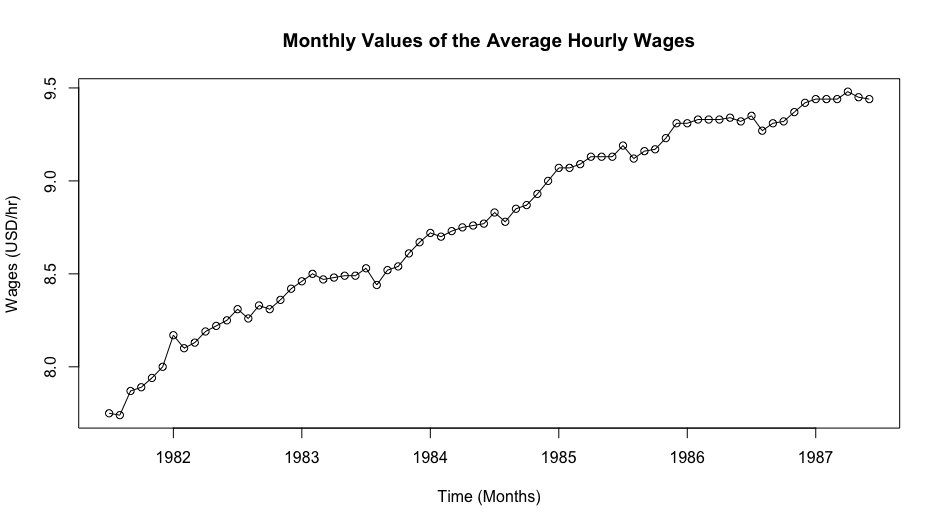
\includegraphics[width=\linewidth]{Images/P1/TS_Plot.png}
        \captionof{figure}[Time series plot of the wages data.]{Time series plot of the wages data. This shows that the wages are mostly increasing and only deviating from this trend in small proportions.}
        \label{fig:p1_ts}
    \end{minipage}
    \item Linear trend model fit summary: \small\begin{block}
Call:
lm(formula = wages ~ time(wages))

Residuals:
     Min       1Q   Median       3Q      Max 
-0.23828 -0.04981  0.01942  0.05845  0.13136 

Coefficients:
              Estimate Std. Error t value Pr(>|t|)    
(Intercept) -5.490e+02  1.115e+01  -49.24   <2e-16 ***
time(wages)  2.811e-01  5.618e-03   50.03   <2e-16 ***
---
Signif. codes:  0 ‘***’ 0.001 ‘**’ 0.01 ‘*’ 0.05 ‘.’ 0.1 ‘ ’ 1

Residual standard error: 0.08257 on 70 degrees of freedom
Multiple R-squared:  0.9728,	Adjusted R-squared:  0.9724 
F-statistic:  2503 on 1 and 70 DF,  p-value: < 2.2e-16
\end{block}
\normalsize
The R\textsuperscript{2} value of this fit is very good ($\approx 0.97$) which signifies that the linear fit is working well. The estimated regression equation is given by Eq \eqref{eq:reg}.
    \begin{equation}
    \label{eq:reg}
        \widehat{X_t} = -549 + 0.2811X_t + \varepsilon
    \end{equation}
    where $\varepsilon \sim \mathcal{N}(0, 0.08257)$ 
    \begin{figure}[!htb]
        \centering
        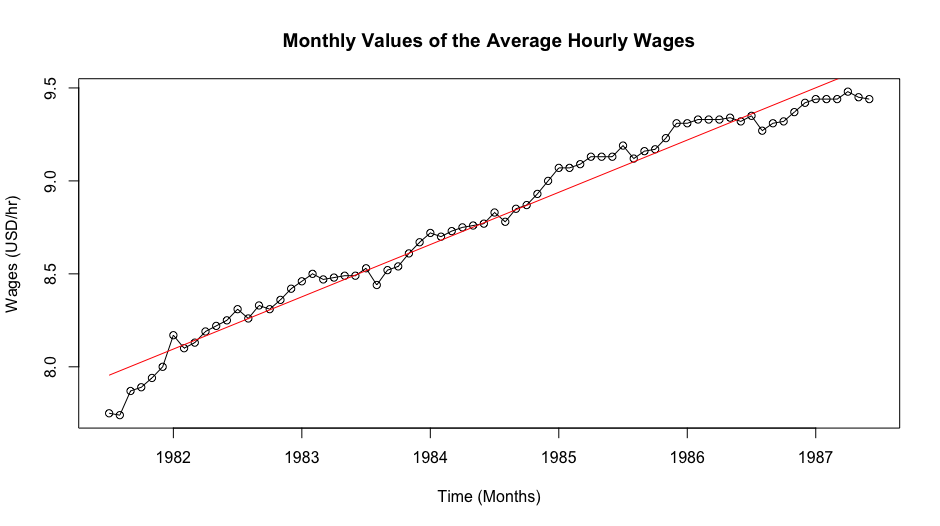
\includegraphics[width=0.9\linewidth]{Images/P1/Linear_Fit.png}
        \caption{Wages plot showing the linear trend in red.}
        \label{fig:lfit}
    \end{figure}
\item 
    \begin{minipage}[!h]{\linewidth}
        \centering
        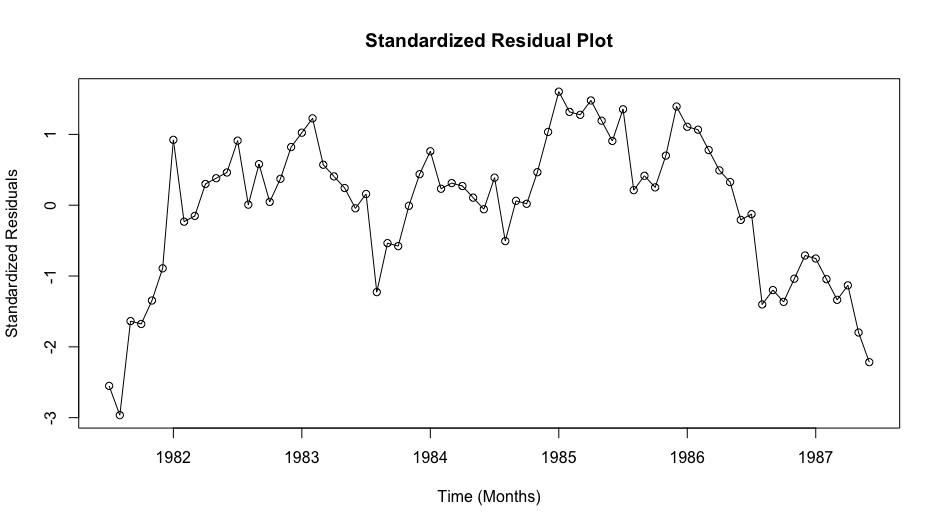
\includegraphics[width=0.9\linewidth]{Images/P1/SR_Plot.png}
        \captionof{figure}[Standardized residuals from the linear regression versus time.]{Standardized residuals from the linear regression versus time. Since the majority of the standardized residuals are within the [-2, 1] interval, so the model residuals strongly follow a normal distribution. Hence, we have a good fit.}
            \label{fig:sr}
    \end{minipage}
\item Quadratic time trend model summary: \small\begin{block}
Call:
lm(formula = wages ~ time(wages) + I(time(wages)^2))

Residuals:
      Min        1Q    Median        3Q       Max 
-0.148318 -0.041440  0.001563  0.050089  0.139839 

Coefficients:
                   Estimate Std. Error t value Pr(>|t|)    
(Intercept)      -8.495e+04  1.019e+04  -8.336 4.87e-12 ***
time(wages)       8.534e+01  1.027e+01   8.309 5.44e-12 ***
I(time(wages)^2) -2.143e-02  2.588e-03  -8.282 6.10e-12 ***
---
Signif. codes:  0 ‘***’ 0.001 ‘**’ 0.01 ‘*’ 0.05 ‘.’ 0.1 ‘ ’ 1

Residual standard error: 0.05889 on 69 degrees of freedom
Multiple R-squared:  0.9864,	Adjusted R-squared:  0.986 
F-statistic:  2494 on 2 and 69 DF,  p-value: < 2.2e-16
\end{block}  
\normalsize
The R\textsuperscript{2} value of this fit is even better ($\approx 0.98$) when compared to the linear fit earlier. This implies that the quadratic trend is more appropriate. The estimated regression equation is given by Eq \eqref{eq:regq}.
    \begin{equation}
    \label{eq:regq}
        \widehat{X_t} = -84950 + 85.34X_t - 0.02143X^2_t + \varepsilon
    \end{equation}
    where $\varepsilon \sim \mathcal{N}(0, 0.05889)$ 
    \begin{figure}[!h]
        \centering
        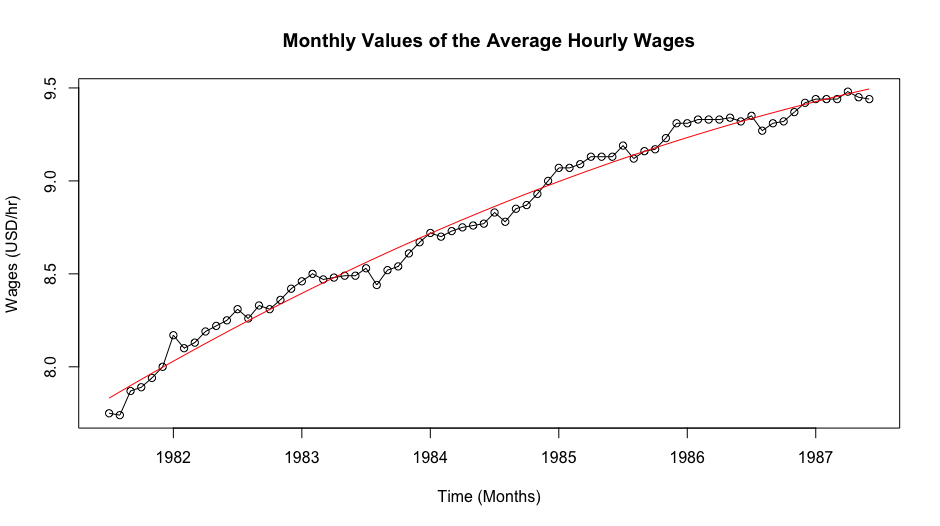
\includegraphics[width=0.9\linewidth]{Images/P1/Q_Fit.png}
        \caption{Wages plot showing the quadratic fit in red.}
        \label{fig:qfit}
    \end{figure}
    \begin{figure}[!h]
        \centering
        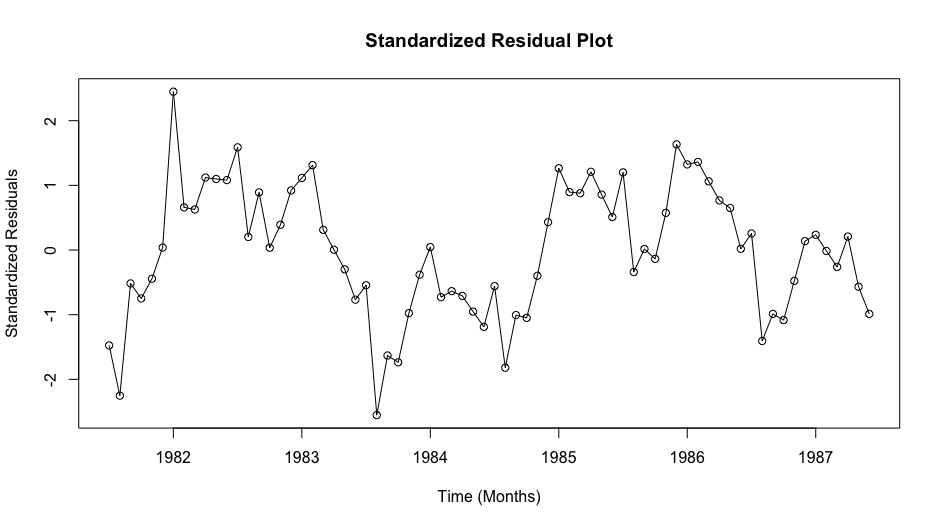
\includegraphics[width=0.9\linewidth]{Images/P1/SR_plot_q.png}
        \caption[Standardized residual plot for the quadratic fit.]{Standardized residual plot for the quadratic fit. Here, we observe that these most of these residuals are in the $\pm2$ region. So, the quadratic fit is better than the linear one.}
        \label{fig:sr_q}
    \end{figure}
\item 
\begin{minipage}[!h]{\linewidth}
    \centering
    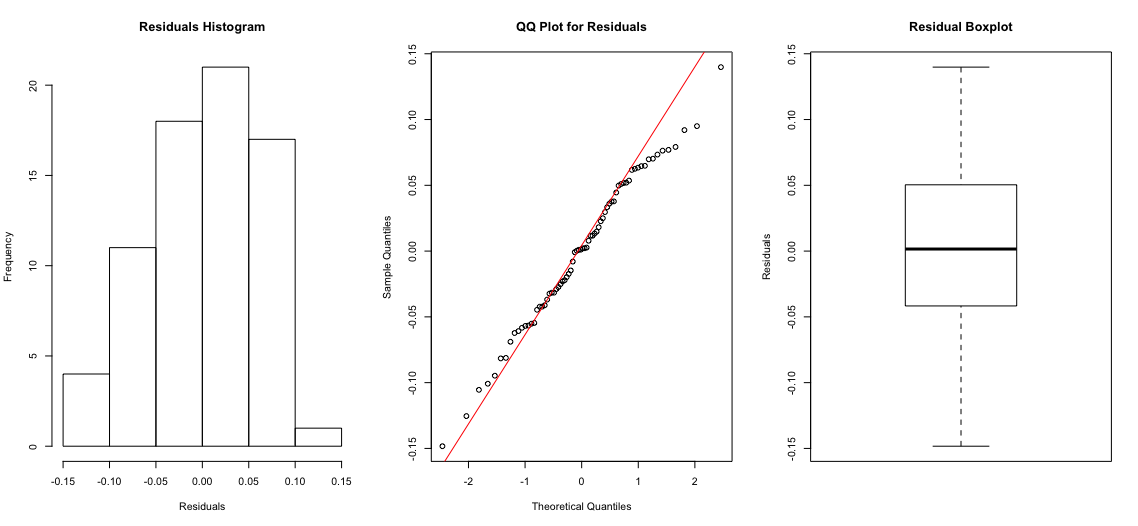
\includegraphics[width=\linewidth]{Images/P1/RD_P1.png}
    \captionof{figure}[Residual diagnostics of the quadratic model.]{Residual diagnostics of the quadratic model showing residual histogram, qq-plot, and boxplot. These plots show that the residuals closely follow a normal distribution.}
    \label{fig:rd_p1}
\end{minipage}
\item \begin{minipage}[!h]{\linewidth}
\centering
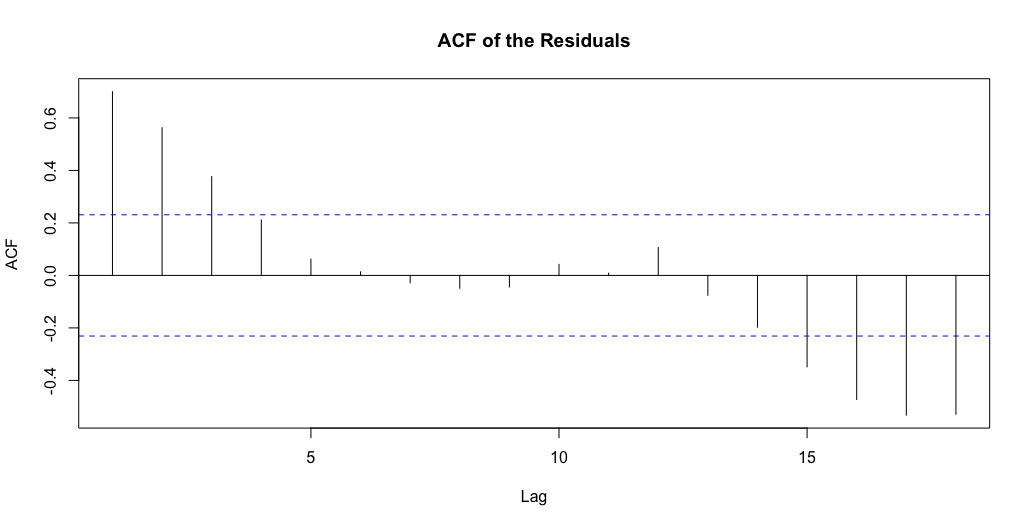
\includegraphics[width=0.9\linewidth]{Images/P1/ACF_P1.png}
\captionof{figure}[Autocorrelation  function (ACF)  for  the  standardized  residuals  from  the  quadratic regression.]{Autocorrelation  function (ACF)  for  the  standardized  residuals  from  the  quadratic regression. This shows that the ACF quickly degrades to zero as the lag increases.}
\end{minipage}
\item Residual normality checks: \small\begin{block}
Shapiro-Wilk normality test
data:  wages.qm$residuals
W = 0.98856, p-value = 0.7622

Exact runs test
data:  wages.qm$residuals
Runs = 15, p-value = 1.284e-07
alternative hypothesis: two.sided
\end{block}
\normalsize
The Shapiro-Wilk test shows that the residuals are normally distributed (p-value $>$ 0.05 and W is close to 1). However, the runs test suggests that the order of the residuals is not random. 
\end{enumerate}